\chapter{Interpreters}\label{ch:interpreters}

\chapquotewl{``When I use a word,'' Humpty Dumpty said, in a rather scornful tone, ``it means just what I choose it to mean - nothing more nor less.'' \\ \hspace*{2em}
``The question is,'' said Alice, ``whether you can make words mean so many different things.''}{Lewis Carroll, \emph{Through the Looking Glass}}{13cm}\index{people}{Carroll, Lewis}

\chapquoter{The tools we use have a profound (and devious!) influence on our\\
thinking habits, and, therefore, on our thinking abilities.}{Edsger Dijkstra, \emph{How do we tell truths that might hurt?}}\index{people}{Dijkstra, Edsger}

\LATER{Second quote about language}

%%% \begin{schemeregion} Cannot be used here, messes up python listings!

Languages are powerful tools for thinking.  Different languages encourage different ways of thinking and lead to different thoughts.  Hence, inventing new languages is a powerful way for solving problems.  We can solve a problem by designing a language in which it is easy to express a solution and implementing an interpreter for that language.  

An \definition{interpreter} is just a program.  As input, it takes a specification of a program in some language.  As output, it produces the output of the input program.  Implementing an interpreter further blurs the line between \emph{data} and \emph{programs}, that we first crossed in Chapter~\ref{ch:programming} by passing procedures as parameters and returning new procedures as results.  Programs are just data input for the interpreter program.  The interpreter determines the meaning of the program.  

To implement an interpreter for a given target language we need to:
\begin{enumtight}
\item Implement a \definition{parser} that takes as input a string representation of a program in the target language and produces a structural parse of the input program.  The parser should break the input string into its language components, and form a parse tree data structure that represents the input text in a structural way.  Section~\ref{sec:parser} describes our parser implementation.  
\item Implement an \definition{evaluator} that takes as input a structural parse of an input program, and evaluates that program.  The evaluator should implement the target language's evaluation rules. Section~\ref{sec:evaluator} describes our evaluator.
\end{enumtight}

Our target language is a simple subset of Scheme we call \emph{Charme}.\footnote{The original name of Scheme was ``Schemer'', a successor to the languages ``Planner'' and ``Conniver''.  Because the computer on which ``Schemer'' was implemented only allowed six-letter file names, its name was shortened to ``Scheme''.  In that spirit, we name our snake-charming language, ``Charmer'' and shorten it to Charme.  Depending on the programmer's state of mind, the language name can be pronounced either ``charm'' or ``char me''.}   The Charme language is very simple, yet is powerful enough to express all computations (that is, it is a universal programming language).  Its evaluation rules are a subset of the stateful evaluation rules for Scheme. The full grammar and evaluation rules for Charme are given in Section~\ref{sec:evaluator}.  The evaluator implements those evaluation rules.  
% Charme includes the application expression, if expression, lambda expression, name expression, and definitions.  It supports integral numbers, and provides the basic arithmetic and comparison primitives with the same meanings as they have in Scheme.  

Section~\ref{sec:laziness} illustrates how changing the evaluation rules of our interpreter opens up new ways of programming.

\section{Python}\label{sec:python}

We could implement a Charme interpreter using Scheme or any other universal programming language, but implement it using the programming language Python.  Python is a popular programming language initially designed by Guido van Rossum in 1991.\footnote{The name \emph{Python} alludes to Monty Python's Flying Circus.}  Python is freely available from \url{http://www.python.org}.  \LATER{What version?}
\cut{
Python is widely used to develop dynamic web applications and as a scripting language for applications.  Python was used to manage special effects production for Star Wars: Episode II, and is used extensively in many organizations including Google, reddit.com, and NASA.\footnote{See \url{http://www.python.org/about/quotes/} for more descriptions of Python uses.}  
}

We use Python instead of Scheme to implement our Charme interpreter for a few reasons.  The first reason is pedagogical: it is instructive to learn new languages. As Dijkstra's quote at the beginning of this chapter observes, the languages we use have a profound effect on how we think.  This is true for natural languages, but also true for programming languages.  Different languages make different styles of programming more convenient, and it is important for every programmer to be familiar with several different styles of programming.  All of the major concepts we have covered so far apply to Python nearly identically to how they apply to Scheme, but seeing them in the context of a different language should make it clearer what the fundamental concepts are and what are artifacts of a particular programming language.  
\sidepicturenocap{1.0}{images/charmer-iStock_000003600257XSmall.jpg}

Another reason for using Python is that it provides some features that enhance expressiveness that are not available in Scheme.  These include built-in support for objects \cut{(as we saw in Chapter~\ref{ch:objects} it is possible to develop an object system for Scheme, but because Scheme does not provide syntactic support for objects is somewhat cumbersome)} and imperative control structures.  Python is also well-supported by most web servers (including Apache), and is widely used to develop dynamic web applications.

The grammar for Python is quite different from the Scheme grammar, so Python programs look very different from Scheme programs.  The evaluation rules, however, are quite similar to the evaluation rules for Scheme.  This chapter does not describe the entire Python language, but introduces the grammar rules and evaluation rules for the most important Python constructs as we use them to implement the Charme interpreter.  \LATER{Pointer to Appendix that is Python reference}\cut{ See \url{http://www.python.org} for more complete documentation on Python.}

% Python comic: http://xkcd.com/353/images/python.png

Like Scheme, Python is a \emph{universal programming language}.  Both languages can express \emph{all} mechanical computations.  For any computation we can express in Scheme, there is a Python program that defines the same computation.  Conversely, every Python program has an equivalent Scheme program.  
\sidepicturenocap{0.4}{images/python-powered-h-140x182.png}

One piece of evidence that every Scheme program has an equivalent Py\-thon program is the interpreter we develop in this chapter.  Since we can implement an interpreter for a Scheme-like language in Python, we know we can express every computation that can be expressed by a program in that language with an equivalent Python program: the Charme interpreter with the Charme program as its input.    

\shortsection{Tokenizing} We introduce Python using one of the procedures in our interpreter implementation.   We divide the job of parsing into two procedures that are combined to solve the problem of transforming an input string into a list describing the input program's structure.  The first part is the \definition{tokenizer}.  It takes as input a string representing a Charme program, and outputs a list of the tokens in that string.  

A \definition{token} is an indivisible syntactic unit.  For example, the Charme expression, 
\scheme|(define square (lambda (x) (* x x)))|, contains 15 tokens: \keyword{(}, \keyword{define}, \keyword{square}, \keyword{(}, \keyword{lambda}, \keyword{(}, \keyword{x}, \keyword{)}, \keyword{(}, \keyword{*}, \keyword{x}, \keyword{x}, \keyword{)}, \keyword{)}, and \keyword{)}.  Tokens are separated by whitespace (spaces, tabs, and newlines).  Punctuation marks such as the left and right parentheses are tokens by themselves.

The \pycode|tokenize| procedure below takes as input a string \pycode|s| in the Charme target language, and produces as output a list of the tokens in \pycode|s|.  We describe the Python language constructs it uses next.\cut{, but attempt to understand it on your own first.}
\begin{pythoncode}
def tokenize(s):   # \sidemark{\# starts a comment until the end of the line}
    current = ' '  # \sidemark{initialize \emph{current} to the empty string (two single quotes)}
    tokens = []    # \sidemark{initialize \emph{tokens} to the empty list}
    for c in s:    # \sidemark{for each character, \emph{c}, in the string \emph{s}}
        if c.isspace():   # \sidemark{if \emph{c} is a whitespace}
            if len(current) > 0:   # \sidemark{if the current token is non-empty}
                tokens.append(current)   # \sidemark{add it to the list}
                current = ''   # \sidemark{reset current token to empty string}
        elif c in '()':   # \sidemark{otherwise, if {\em c} is a parenthesis}
            if len(current) > 0:   # \sidemark{end the current token}
                tokens.append(current)   # \sidemark{add it to the tokens list}
                current = ' '  # \sidemark{and reset {\em current} to the empty string}
            tokens.append(c)   # \sidemark{add the parenthesis to the token list}
        else:   # \sidemark{otherwise (it is an alphanumeric)}
            current = current + c   # \sidemark{add the character to the current token}
    # end of the for loop \sidemark{reached the end of {\em s}}
    if len(current) > 0:   # \sidemark{if there is a current token}
        tokens.append(current)   # \sidemark{add it to the token list}
    return tokens   # \sidemark{the result is the list of tokens}
\end{pythoncode}

\subsection{Python Programs}

Whereas Scheme programs are composed of expressions and definitions, Python programs are mostly sequences of statements.  Unlike expressions, a statement has no value.  The emphasis on statements impacts the style of programming used with Python.  It is more imperative than that used with Scheme: instead of composing expressions in ways that pass the result of one expression as an operand to the next expression, Python procedures consist mostly of statements, each of which alters the state in some way towards reaching the goal state.  Nevertheless, it is possible (but not recommended) to program in Scheme using an imperative style (emphasizing assignments), and it is possible (but not recommended) to program in Python using a functional style (emphasizing procedure applications and eschewing statements).

Defining a procedure in Python is similar to defining a procedure in Scheme, except the syntax is different:
\begin{bnfgrammarm}{ProcedureDefinition}
\bnfrule{ProcedureDefinition}{\terminal{def} \terminal{\emph{Name}} \terminal{\lparen} \nonterminal{Parameters} \terminal{\rparen} \terminal{:} \nonterminal{Block}}
\bnfrule{Parameters}{$\epsilon$}
\bnfrule{Parameters}{\nonterminal{SomeParameters}}
\bnfrule{SomeParameters}{\terminal{\emph{Name}}}
\bnfrule{SomeParameters}{\terminal{\emph{Name}} \terminal{,} \nonterminal{SomeParameters}}
\ \\
\bnfrule{Block}{\nonterminal{Statement}}
\bnfrule{Block}{\terminal{$<$newline$>$} \emph{indented}\lparen\nonterminal{Statements}\rparen}
\bnfrule{Statements}{\nonterminal{Statement} \terminal{$<$newline$>$} \nonterminal{MoreStatements}}
\bnfrule{MoreStatements}{\nonterminal{Statement} \terminal{$<$newline$>$} \nonterminal{MoreStatements}}
\bnfrule{MoreStatements}{$\epsilon$}
\end{bnfgrammarm}

Unlike in Scheme, whitespace (such as new lines) has meaning in Python. Statements cannot be separated into multiple lines, and only one statement may appear on a single line. Indentation within a line also matters. Instead of using parentheses to provide code structure, Python uses the indentation to group statements into blocks. The Python interpreter reports an error if the indentation does not match the logical structure of the code.

Since whitespace matters in Python, we include newlines (\terminal{$<$newline$>$}) and indentation in our grammar.  We use \emph{indented}(\emph{elements})
to indicate that the \emph{elements} are indented.  For example, the rule for \nonterminal{Block} is a newline, followed by one or more statements.  The statements are all indented one level inside the block's indentation.  The block ends when the indenting returns to the outer level.

The evaluation rule for a procedure definition is similar to the rule for evaluating a procedure definition in Scheme.
\mevalrule{Python Procedure Definition}{The procedure definition, 
\begin{smallquote}
\terminal{def} \terminal{\emph{Name}} \terminal{\lparen}{\nonterminal{Parameters}}\terminal{\rparen}\terminal{:} \nonterminal{Block}
\end{smallquote}
defines \terminal{\emph{Name}} as a procedure that takes as inputs the \nonterminal{Parameters} and has the body expression \nonterminal{Block}.} 

The procedure definition, \pycode|def tokenize(s): ...|, defines a procedure named \pycode|tokenize| that takes a single parameter, \pycode|s|.  

\shortsection{Assignment} \index{general}{assignment}The body of the procedure uses several different types of Python statements.  Following Python's more imperative style, five of the statements in \pycode|tokenize| are assignment statements including the first two statements.  For example, the assignment statement, \pycode|tokens = []| assigns the value \pycode|[]| (the empty list) to the name \pycode|tokens|.

The grammar for the assignment statement is:
\begin{bnfgrammarm}{AssignmentStatement}
\bnfrule{Statement}{\nonterminal{AssignmentStatement}}
\bnfrule{AssignmentStatement}{\nonterminal{Target} \terminal{=} \nonterminal{Expression}}
\bnfrule{Target}{\terminal{\emph{Name}}}
\end{bnfgrammarm}
For now, we use only a \emph{Name} as the left side of an assignment, but since other constructs can appear on the left side of an assignment statement, we introduce the nonterminal \nonterminal{Target} for which additional rules can be defined to encompass other possible assignees.  Anything that can hold a value (such as an element of a list) can be the target of an assignment.

The evaluation rule for an assignment statement is similar to Scheme's evaluation rule for assignments: the meaning of \pycode|x = e| in Python is similar to the meaning of \scheme|(set! x e)| in Scheme, except that in Python the target \emph{Name} need not exist before the assignment.  In Scheme, it is an error to evaluate \scheme|(set! x 7)| where the name \scheme|x| has not been previously defined; in Python, if \pycode|x| is not already defined, evaluating \pycode|x = 7| creates a new place named \pycode|x| with its value initialized to \pycode|7|.

\mevalrule{Python Evaluation Rule: Assignment}{To evaluate an assignment statement, evaluate the expression, and assign the value of the expression to the place identified by the target.  If no such place exists, create a new place with that name.}

\shortsection{Arithmetic and Comparison Expressions}  Python supports many different kinds of expressions for performing arithmetic and comparisons.  Since Python does not use parentheses to group expressions, the grammar provides the grouping by breaking down expressions in several steps.  This defines an order of \definition{precedence} for parsing expressions. 
% If a complex expression includes many expressions, the grammar specifies how they will be grouped.  

For example, consider the expression \pycode|3 + 4 * 5|.  In Scheme, the expressions \scheme|(+ 3 (* 4 5))| and \scheme|(* (+ 3 4) 5)| are clearly different and the parentheses group the subexpressions.  The Python expression, \pycode|3 + 4 * 5|, means \scheme|(+ 3 (* 4 5))| and evaluates to \presult|23|.  %The expression \pycode|4 * 5 + 3| also evaluates to \presult|23|.  

Supporting precedence makes the Python grammar rules more complex since they must deal with \pycode|*| and \pycode|+| differently, but it makes the meaning of Python expressions match our familiar mathematical interpretation, without needing to clutter expressions with parentheses.  This is done is by defining the grammar rules so an \nonterminal{AddExpression} can contain a \nonterminal{MultExpression} as one of its subexpressions, but a \nonterminal{MultExpression} cannot contain an \nonterminal{AddExpression}.  This makes the multiplication operator have \emph{high\-er pre\-ce\-dence} than the addition operator.  If an expression contains both \pycode|+| and \pycode|*| operators, the \pycode|*| operator is grouped with its operands first.  The replacement rules that happen first have lower precedence, since their components must be built from the remaining pieces. 

Here are the grammar rules for Python expressions for comparison, multiplication, and addition expressions:
\begin{bnfgrammarm}{PrimaryExpression}
\bnfrule{Expression}{\nonterminal{CompExpr}}
\bnfrule{CompExpr}{\nonterminal{CompExpr} \nonterminal{Comparator} \nonterminal{CompExpr}}
\bnfrule{Comparator}{\terminal{$<$} $\mid$ \terminal{$>$} $\mid$ \terminal{==} $\mid$ \terminal{$<$=} $\mid$ \terminal{$>$=}}
\bnfrule{CompExpr}{\nonterminal{AddExpression}}
\end{bnfgrammarm}

\begin{bnfgrammarm}{PrimaryExpression}
\bnfrule{AddExpression}{\nonterminal{AddExpression} \terminal{+} \nonterminal{MultExpression}}
\bnfrule{AddExpression}{\nonterminal{AddExpression} \terminal{-} \nonterminal{MultExpression}}
\bnfrule{AddExpression}{\nonterminal{MultExpression}}
\end{bnfgrammarm}

\begin{bnfgrammarm}{PrimaryExpression}
\bnfrule{MultExpression}{\nonterminal{MultExpression} \terminal{*} \nonterminal{PrimaryExpression}}
\bnfrule{MultExpression}{\nonterminal{PrimaryExpression}}
\end{bnfgrammarm}

\begin{bnfgrammarm}{PrimaryExpression}
\bnfrule{PrimaryExpression}{\nonterminal{Literal}}
\bnfrule{PrimaryExpression}{\terminal{\emph{Name}}}
\bnfrule{PrimaryExpression}{\terminal{\lparen} \nonterminal{Expression} \terminal{\rparen}}
\end{bnfgrammarm}
The last rule allows expressions to be grouped explicitly using parentheses.  For example, \pycode|(3 + 4) * 5| is parsed as the \nonterminal{PrimaryExpression}, \pycode|(3 + 4)|, times \pycode|5|, so evaluates to \presult|35|; without the parentheses, \pycode|3 + 4 * 5| is parsed as \pycode|3| plus the \nonterminal{MultExpression}, \pycode|4 * 5|, so evaluates to \pycode|23|.

A \nonterminal{PrimaryExpression} can be a \nonterminal{Literal}, such as a number.  Numbers in Python are similar (but not identical) to numbers in Scheme.  %In the example program, we use the integer literal \pycode|0|.  

A \nonterminal{PrimaryExpression} can also be a name, similar to names in Scheme.  The evaluation rule for a name in Python is similar to the stateful rule for evaluating a name in Scheme\footnote{There are some subtle differences and complexities (see Section 4.1 of the Python Reference Manual), however, which we do not go into here.}.

\beforeex
\begin{exercise}
Draw the parse tree for each of the following Python expressions and provide the value of each expression.
\begin{subexerciselist}
\item \pycode|1 + 2 + 3 * 4|
\solution{\LATER{}}
\item \pycode|3 > 2 + 2|
\solution{\LATER{}}
\item \pycode|3 * 6 >= 15 == 12|
\solution{\LATER{}}
\item \pycode|(3 * 6 >= 15) == True|
\solution{\LATER{}}
\end{subexerciselist}
\end{exercise}
\afterex

\beforeex
\begin{exercise}
Do comparison expressions have higher or lower precedence than addition expressions?  Explain why using the grammar rules.
\solution{\LATER{}}
\end{exercise}
\afterex


\subsection{Data Types}\label{sec:pythonlists}

Python provides many built-in data types.  We describe three of the most useful data types here: lists, strings, and dictionaries.

\shortsection{Lists} \index{general}{List (Python)} Python provides a list datatype similar to lists in Scheme, except instead of building lists from simpler parts (that is, using \scheme|cons| pairs in Scheme), the Python list type is a built-in datatype.  The other important difference is that Python lists are mutable like \scheme|mlist| from Section~\ref{sec:mutablepairs}.

Lists are denoted in Python using square brackets.  For example, \pycode|[]| denotes an empty list and \pycode|[1, 2]| denotes a list containing two elements.  The elements in a list can be of any type (including other lists).

Elements can be selected from a list using the list subscript expression:
\begin{bnfgrammarm}{SubscriptExpression}
\bnfrule{PrimaryExpression}{\nonterminal{SubscriptExpression}}
\bnfrule{SubscriptExpression}{\nonterminal{PrimaryExpression} \terminal{[} \nonterminal{Expression} \terminal{]}}
\end{bnfgrammarm}
%If the first primary expression evaluates to a list, t
A subscript expression evaluates to the element indexed by value of the inner expression from the list.  For example,

\begin{pythoninteracts}
\pyn{a = [1, 2, 3]}
\pyi{a[0]}{1}
\pyi{a[1+1]}{3}
\pye{a[3]}{IndexError: list index out of range}
\end{pythoninteracts}

The expression \pycode|p[0]| in Python is analogous to \scheme|(car p)| in Scheme.

%Negative selection indexes select elements from the back of the list.  The expression \pycode|p[-1]| selects the last element in the list \pycode|p|.

The subscript expression has constant running time; unlike indexing Scheme lists, the time required does not depend on the length of the list even if the selection index is the end of the list.  The reason for this is that Python stores lists internally differently from how Scheme stores as chains of pairs.  The elements of a Python list are stored as a block in memory, so the location of the $k^{th}$ element can be calculated directly by adding $k$ times the size of one element to the location of the start of the list.  

A subscript expression can also select a range of elements from the list:
\begin{bnfgrammarm}{SubscriptExpression}
\bnfrule{SubscriptExpression}{\nonterminal{PrimaryExpression} \terminal{[} \nonterminal{Bound$_{Low}$} \terminal{:} \nonterminal{Bound$_{High}$} \terminal{]}}
\bnfrule{Bound}{\nonterminal{Expression} $\mid$ $\epsilon$}
\end{bnfgrammarm}

Subscript expressions with ranges evaluate to a list containing the elements between the low bound and the high bound.  If the low bound is missing, the low bound is the beginning of the list.  If the high bound is missing, the high bound is the end of the list.  For example,

\begin{pythoninteracts}
\pyn{a = [1, 2, 3]}
\pyi{a[:1]}{[1]}
\pyi{a[1:]}{[2, 3]}
\pyi{a[4-2:3]}{[3]}
\pyi{a[:]}{[1, 2, 3]}
\end{pythoninteracts}

The expression \pycode|p[1:]| in Python is analogous to \scheme|(cdr p)| in Scheme.

Python lists are mutable (the value of a list can change after it is created).  We can use list subscripts as the targets for an assignment expression:
\begin{bnfgrammarm}{Target}
\bnfrule{Target}{\nonterminal{SubscriptExpression}}
\end{bnfgrammarm}
Assignments using ranges as targets can add elements to the list as well as changing the values of existing elements:

\begin{pythoninteracts}
\pyn{a = [1, 2, 3]}
\pyn{a[0] = 7}
\pyi{a}{[7, 2, 3]}
\pyn{a[1:4] = [4, 5, 6]}
\pyi{a}{[7, 4, 5, 6]}
\pyn{a[1:] = [6]}
\pyi{a}{[7, 6]}
\end{pythoninteracts}

In the \pycode|tokenize| procedure, we use \pycode|tokens = []| to initialize \pycode|tokens| to an empty list, and use \pycode|tokens.append(current)| to append an element to the \pycode|tokens| list.  The Python \pycode|append| procedure is similar to the \scheme|mlist-append!| procedure (except it works on the empty list, where there is no way in Scheme to modify the null input list).

\shortsection{Strings}\index{general}{string} The other datatype used in \pycode|tokenize| is the string datatype, named \pycode|str| in Python.  As in Scheme, a String is a sequence of characters.  Unlike Scheme strings  which are mutable, the Python \pycode|str| datatype is immutable.  Once a string is created its value cannot change.  This means all the string methods that seem to change the string values actually return new strings (for example, \pycode|capitalize()| returns a copy of the string with its first letter capitalized). 
% The value of a variable that is a string can change by assigning a new string object to that variable, but this does not change the value of the original string object.

Strings can be enclosed in single quotes (e.g., \pycode|'hello'|), double quotes (e.g., \pycode|''hello''|), and triple-double quotes (e.g., \pycode|'' '' ''hello'' '' ''|; a string inside triple quotes can span multiple lines).  In our example program, we use the assignment expression, \pycode|current = ' '| (two single quotes), to initialize the value of \pycode|current| to the empty string.   The input, \pycode|s|, is a string object.

The addition operator can be used to concatenate two strings.  In \pycode|tokenize|, we use \pycode|current = current + c| to update the value of \pycode|current| to include a new character.  Since strings are immutable there is no string method analogous to the list \pycode|append| method.  Instead, appending a character to a string involves creating a new string object.

\shortsection{Dictionaries}\index{general}{dictionary}  A dictionary is a lookup-table where values are associated with keys.  The keys can be any immutable type (strings and numbers are commonly used as keys); the values can be of any type.  We did not use the dictionary type in \pycode|tokenize|, but it is very useful for implementing frames in the evaluator.

A dictionary is denoted using curly brackets.  The empty dictionary is \pycode|{}|.  We add a key-value pair to the dictionary using an assignment where the left side is a subscript expression that specifies the key and the right side is the value assigned to that key.  For example,
\begin{pythoncode}
birthyear = {} 
birthyear['Euclid'] = '300BC'
birthyear['Ada'] = 1815
birthyear['Alan Turing'] = 1912
birthyear['Alan Kay'] = 1940
\end{pythoncode}
defines \pycode|birthyear| as a dictionary containing four entries.  The keys are all strings; the values are numbers, except for Euclid's entry which is a string.

We can obtain the value associated with a key in the dictionary using a subscript expression.  For example, \pycode|birthyear['Alan Turing']| evaluates to \pycode|1912|.  We can replace the value associated with a key using the same syntax as adding a key-value pair to the dictionary.  The statement,
\begin{pythoncode}
birthyear['Euclid'] = -300
\end{pythoncode}
replaces the value of \pycode|birthyear['Euclid']| with the number \pycode|-300|.

The dictionary type also provides a method \pycode|has_key| that takes one input and produces a Boolean indicating if the dictionary object contains the input value as a key.  For the \pycode|birthyear| dictionary, 

\begin{pythoninteractsm}{birthyear.has_key('John Backus')}
\pyi{birthyear.has_key('John Backus')}{False}
\pyi{birthyear.has_key('Ada')}{True}
\end{pythoninteractsm}

The dictionary type lookup and update operations have approximately constant running time: the time it takes to lookup the value associated with a key does not scale as the size of the dictionary increases.  This is done by computing a number based on the key that determines where the associated value would be stored (if that key is in the dictionary).  The number is used to index into a structure similar to a Python list (so it has constant time to retrieve any element).  Mapping keys to appropriate numbers to avoid many keys mapping to the same location in the list is a difficult problem, but one the Python dictionary object does well for most sets of keys.

\subsection{Applications and Invocations}\index{general}{Objects (Python)}\index{general}{Methods (Python)}

The grammar rules for expressions that apply procedures are:

\begin{bnfgrammarm}{PrimaryExpression}
\bnfrule{PrimaryExpression}{\nonterminal{CallExpression}}
\bnfrule{CallExpression}{\nonterminal{PrimaryExpression} \terminal{\lparen} \nonterminal{ArgumentList} \terminal{\rparen}}
\bnfrule{ArgumentList}{\nonterminal{SomeArguments}}
\bnfrule{ArgumentList}{$\epsilon$}
\bnfrule{SomeArguments}{\nonterminal{Expression}}
\bnfrule{SomeArguments}{\nonterminal{Expression} \terminal{,} \nonterminal{SomeArguments}}
\end{bnfgrammarm}

In Python, nearly every data value (including lists and strings) is an object.  This means the way we manipulate data is to invoke methods on objects.  To invoke a method we use the same rules, but the \nonterminal{PrimaryExpression} of the \nonterminal{CallExpression} specifies an object and method:
\begin{bnfgrammarm}{AttributeReference}
\bnfrule{PrimaryExpression}{\nonterminal{AttributeReference}}
\bnfrule{AttributeReference}{\nonterminal{PrimaryExpression} \terminal{.} \terminal{\emph{Name}}}
\end{bnfgrammarm}

The name \nonterminal{AttributeReference} is used since the same syntax is used for accessing the internal state of objects as well.

The \pycode|tokenize| procedure includes five method applications, four of which are \pycode|tokens.append(current)|.  The object reference is \pycode|tokens|, the list of tokens in the input.  The list \pycode|append| method takes one parameter and adds that value to the end of the list.  

The other method invocation is \pycode|c.isspace()| where \pycode|c| is a string consisting of one character in the input.  The \pycode|isspace| method for the string datatype returns true if the input string is non-empty and all characters in the string are whitespace (either spaces, tabs, or newlines).  

The \pycode|tokenize| procedure also uses the built-in function \pycode|len| which takes as input an object of a collection datatype such as a list or a string, and outputs the number of elements in the collection.  It is a procedure, not a method; the input object is passed in as a parameter.  In \pycode|tokenize|, we use \pycode|len(current)| to find the number of characters in the current token.  

\subsection{Control Statements}

Python provides control statements for making decisions, looping, and for returning from a procedure.

\shortsection{If statement} Python's if statement is similar to the conditional expression in Scheme:

\begin{bnfgrammarm}{IfStatement}
\bnfrule{Statement}{IfStatement}
\bnfrule{IfStatement}{\terminal{if} \nonterminal{Expression$_{Predicate}$} \terminal{:} \nonterminal{Block} \nonterminal{Elifs} \nonterminal{OptElse}}
\bnfrule{Elifs}{$\epsilon$}
\bnfrule{Elifs}{\terminal{elif} \nonterminal{Expression$_{Predicate}$} \terminal{:} \nonterminal{Block} \nonterminal{Elifs}}
\bnfrule{OptElse}{$\epsilon$}
\bnfrule{OptElse}{\terminal{else} \terminal{:} \nonterminal{Block}}
\end{bnfgrammarm}

Unlike in Scheme, there is no need to have an alternate clause since the Python if statement does not need to produce a value.  %Hence, the \pycode|else| is optional.
The evaluation rule is similar to Scheme's conditional expression: 

\mevalrule{Python Evaluation Rule: If}{First, evaluate the \nonterminal{Expression$_{Predicate}$}.  If it evaluates to a true value, the consequent \nonterminal{Block} is evaluated, and none of the rest of the \nonterminal{IfStatement} is evaluated.  Otherwise, each of the \nonterminal{elif} predicates is evaluated in order.  If one evaluates to a true value, its \nonterminal{Block} is evaluated and none of the rest of the \nonterminal{IfStatement} is evaluated.  If none of the \nonterminal{elif} predicates evaluates to a true value, the \terminal{else} \nonterminal{Block} is evaluated if there is one.}

The main if statement in \pycode|tokenize| is:
\begin{pythoncode}
if c.isspace(): ...
elif c in '()': ...
else: current = current + c
\end{pythoncode}
The first if predicate tests if the current character is a space.  If so, the end of the current token has been reached.  The consequent \nonterminal{Block} is itself an \nonterminal{IfStatement}:
\begin{pythoncode}
if len(current) > 0: 
   tokens.append(current)
   current = ' ' 
\end{pythoncode}
If the current token has at least one character, it is appended to the list of tokens in the input string and the current token is reset to the empty string.  This \nonterminal{IfStatement} has no \nonterminal{elif} or \nonterminal{else} clauses, so if the predicate is false, there is nothing to do.  

\cut{If the predicate for the main if statement is false, evaluation proceeds to the \nonterminal{elif} clause.  The predicate for this clause tests if \pycode|c| is in the set of characters given by the literal string \pycode|'()'|.  It evaluates to \pycode|true| if \pycode|c| is either an open or close parentheses.  As with spaces, a parenthesis ends the previous token, so the first statement in the \nonterminal{elif} clauses is identical to the first consequent clause.  The difference is unlike spaces, we need to keep track of the parentheses, so it is added to the token list by \pycode|tokens.append(c)|.  

The final clause is an \nonterminal{else} clause, so its body will be evaluated if neither the \pycode|if| or \pycode|elif| predicate is true.  This means the current character is not a space or a parenthesis, so it is some other character which should be added to the current token.  This is done by the assignment expression, \pycode|current = current + c|.  The addition operator in Python works on strings as well as numbers (and some other datatypes).  For strings, it concatenates the operands into a new string.  Since strings are immutable there is no string method analogous to the list \pycode|append| method.  Instead, appending a character to a string involves creating a new string object.
}

\shortsection{For statement}  A \pycode|for| statement provides a way of iterating through a set of values, carrying out a body block for each value.  
\begin{bnfgrammarm}{ForStatement}
\bnfrule{Statement}{ForStatement}
\bnfrule{ForStatement}{\terminal{for} \nonterminal{Target} \terminal{in} \nonterminal{Expression} \terminal{:} \nonterminal{Block}}
\end{bnfgrammarm}
Its evaluation rule is:
\mevalrule{Python Evaluation Rule: For}{First evaluate the \nonterminal{Expression} which must produce a value that is a collection.  Then, for each value in the collection assign the \nonterminal{Target} to that value and evaluate the \nonterminal{Block}.}

Other than the first two initializations, and the final two statements, the bulk of the \pycode|tokenize| procedure is contained in a \pycode|for| statement.  The for statement in \pycode|tokenize| header is \pycode|for c in s: ...|.  The string \pycode|s| is the input string, a collection of characters.  So, the loop will repeat once for each character in \pycode|s|, and the value of \pycode|c| is each character in the input string (represented as a singleton string), in turn.  

\shortsection{Return statement} In Scheme, the body of a procedure is an expression and the value of that expression is the result of evaluating an application of the procedure.  In Python, the body of a procedure is a block of one or more statements.  Statements have no value, so there is no obvious way to decide what the result of a procedure application should be.  Python's solution is to use a \emph{return statement}.  

The grammar for the return statement is:
\begin{bnfgrammarm}{ReturnStatement}
\bnfrule{Statement}{ReturnStatement}
\bnfrule{ReturnStatement}{\terminal{return} \nonterminal{Expression}}
\end{bnfgrammarm}
A return statement finishes execution of a procedure, returning the value of the \nonterminal{Expression} to the caller as the result.  The last statement of the \pycode|tokenize| procedure is: \pycode|return tokens|.  It returns the value of the \pycode|tokens| list to the caller.

\section{Parser}\label{sec:parser}\index{general}{parsing}

The parser takes as input a Charme program string, and produces as output a nested list that encodes the structure of the input program. The first step is to break the input string into tokens; this is done by the \pycode|tokenize| procedure defined in the previous section.  

The next step is to take the list of tokens and produce a data structure that encodes the structure of the input program.  Since the Charme language is built from simple parenthesized expressions, we can represent the parsed program as a list.  But, unlike the list returned by \pycode|tokenize| which is a flat list containing the tokens in order, the list returned by \pycode|parse| is a structured list that may have lists (and lists of lists, etc.) as elements.  

Charme's syntax is very simple, so the parser can be implemented by just breaking an expression into its components using the parentheses and whitespace.  The parser needs to balance the open and close parentheses that enclose expressions.  For example, if the input string is 
\begin{schemedisplay}
(define square (lambda (x) (* x x)))
\end{schemedisplay}
the output of \pycode|tokenizer| is the list:
\begin{pythoncode}
['(', 'define', 'square', '(', 'lambda', '(', 'x', ')', '(', '*', 'x', 'x', ')', ')', ')']
\end{pythoncode}
The parser structures the tokens according to the program structure, producing a parse tree that encodes the structure of the input program.  The parenthesis provide the program structure, so are removed from the parse tree.  For the example, the resulting parse tree is:
\begin{pythoncode}
['define', 
 'square', 
 [  'lambda', 
    ['x'], 
    ['*', 'x', 'x'] ] ]
\end{pythoncode}
%The output parse structure is a list containing three elements, the first is the keyword \pycode|'define'|, the second is the name \pycode|'square'|, and the third is a list containing three elements, \pycode|['lambda', ['x'], ['*', 'x', 'x']]|, the third of which is itself a list containing three elements.
%%\clearpage %!!!
Here is the definition of \pycode|parse|:
\begin{pythoncode}
def parse(s):
    def parse_tokens(tokens, inner):
       res = []
       while len(tokens) > 0:
          current = tokens.pop(0)
          if current == '(':
             res.append (parse_tokens(tokens, True))
          elif current == ')':
             if inner: return res
             else:
                error('Unmatched close paren: ' + s)
                return None
          else: 
             res.append(current)
        
       if inner:
          error ('Unmatched open paren: ' + s)
          return None
       else:
          return res

    return parse_tokens(tokenize(s), False)
\end{pythoncode}

The input to \pycode|parse| is a string in the target language.  The output is a list of the parenthesized expressions in the input.  Here are some examples:
\begin{pythoninteractsm}{parse('(+ 1 2) (+ 3 4)')}
\pyi{parse('150')}{['150']}
\pyi{parse('(+ 1 2)')}{[['+', '1', '2']]}
\pyi{parse('(+ 1 (* 2 3))')}{[['+', '1', ['*', '2', '3']]]}
\pyl{parse('(define square (lambda (x) (* x x)))')}{[['define', 'square', ['lambda', ['x'], ['*', 'x', 'x']]]]}
\pyi{parse('(+ 1 2) (+ 3 4)')}{[['+', '1', '2'], ['+', '3', '4']]}
\end{pythoninteractsm}

The parentheses are no longer included as tokens in the result, but their presence in the input string determines the structure of the result.

\index{general}{recursive descent}The \pycode|parse| procedure implements a \definition{recursive descent} parser.  The main \pycode|parse| procedure defines the \pycode|parse_tokens| helper procedure and returns the result of calling it with inputs that are the result of tokenizing the input string and the Boolean literal \pycode|False|: \pycode|return parse_tokens(tokenize(s), False)|.  

The \pycode|parse_tokens| procedure takes two inputs: \pycode|tokens|, a list of tokens (that results from the \pycode|tokenize| procedure); and \pycode|inner|, a Boolean that indicates whether the parser is inside a parenthesized expression.  The value of \pycode|inner| is \pycode|False| for the initial call since the parser starts outside a parenthesized expression.  All of the recursive calls result from encountering a \pycode|'('|, so the value passed as \pycode|inner| is \pycode|True| for all the recursive calls.

The body of the \pycode|parse_tokens| procedure initializes \pycode|res| to an empty list that is used to store the result.  Then, the \pycode|while| statement iterates as long as the token list contains at least one element.  

The first statement of the \pycode|while| statement block assigns \pycode|tokens.pop(0)| to \pycode|current|.  The \pycode|pop| method of the list takes a parameter that selects an element from the list.  The selected element is returned as the result.  The \pycode|pop| method also mutates the list object by removing the selected element.  So, \pycode|tokens.pop(0)| returns the first element of the \pycode|tokens| list and removes that element from the list.  This is essential to the parser making progress: every time the \pycode|tokens.pop(0)| expression is evaluated the number of elements in the token list is reduced by one.  

If the \pycode|current| token is an open parenthesis, \pycode|parse_tokens| is called recursively to parse the inner expression (that is, all the tokens until the matching close parenthesis).  The result is a list of tokens, which is appended to the result.  If the \pycode|current| token is a close parenthesis, the behavior depends on whether or not the parser is parsing an inner expression.  If it is inside an expression (that is, an open parenthesis has been encountered with no matching close parenthesis yet), the close parenthesis closes the inner expression, and the result is returned.  If it is not in an inner expression, the close parenthesis has no matching open parenthesis so a parse error is reported.  

The \pycode|else| clause deals with all other tokens by appending them to the list.

The final if statement checks that the parser is not in an inner context when the input is finished.  This would mean there was an open parenthesis without a corresponding close, so an error is reported.  Otherwise, the list representing the parse tree is returned.

\section{Evaluator}\label{sec:evaluator}\index{general}{evaluator}

The evaluator takes a list representing the parse tree of a Charme expression or definition and an environment, and outputs the result of evaluating the expression in the input environment.  The evaluator implements the evaluation rules for the target language.

The core of the evaluator is the procedure \pycode|meval|:

\begin{pythoncode}
def meval(expr, env):
    if is_primitive(expr): return eval_primitive(expr)
    elif is_if(expr): return eval_if(expr, env) 
    elif is_definition(expr): eval_definition(expr, env)
    elif is_name(expr): return eval_name(expr, env)
    elif is_lambda(expr): return eval_lambda(expr, env)
    elif is_application(expr): return eval_application(expr, env)
    else: error ('Unknown expression type: ' + str(expr))
\end{pythoncode}

The if statement matches the input expression with one of the expression types (or the definition) in the Charme language, and returns the result of applying the corresponding evaluation procedure (if the input is a definition, no value is returned since definitions do not produce an output value).  We next consider each evaluation rule in turn.

\subsection{Primitives}\index{general}{primitives}

Charme supports two kinds of primitives: natural numbers and primitive procedures.  If the expression is a number, it is a string of digits.  The \pycode|is_number| procedure evaluates to \pycode|True| if and only if its input is a number:

\begin{pythoncode}
def is_primitive(expr):
    return is_number(expr) or is_primitive_procedure(expr)

def is_number(expr):
    return isinstance(expr, str) and expr.isdigit()
\end{pythoncode}
Here, we use the built-in function \pycode|isinstance| to check if \pycode|expr| is of type \pycode|str|.  The and expression in Python evaluates similarly to the Scheme \pycode|and| special form: the left operand is evaluated first; if it evaluates to a false value, the value of the and expression is that false value.  If it evaluates to a true value, the right operand is evaluated, and the value of the and expression is the value of its right operand.  This evaluation rule means it is safe to use \pycode|expr.isdigit()| in the right operand, since it is only evaluated if the left operand evaluated to a true value, which means \pycode|expr| is a string.  

Primitive procedures are defined using Python procedures.  We define the procedure \pycode|is_primitive_procedure| using \pycode|callable|, a procedure that returns true only for callable objects such as procedures and methods:
\begin{pythoncode}
def is_primitive_procedure(expr):
    return callable(expr)
\end{pythoncode}

The evaluation rule for a primitive is identical to the Scheme rule:

\mevalrule{Charme Evaluation Rule 1: Primitives}{A primitive expression evaluates to its pre-defined value.}

We need to implement the \emph{pre-defined} values in our Charme interpreter.

To evaluate a number primitive, we need to convert the string representation to a number of type \pycode|int|.  The \pycode|int(s)| constructor takes a string as its input and outputs the corresponding integer:

\begin{pythoncode}
def eval_primitive(expr):
    if is_number(expr): return int(expr)
    else: return expr
\end{pythoncode}

The \pycode|else| clause means that all other primitives (in Charme, this is only primitive procedures and Boolean constants) self-evaluate: the value of evaluating a primitive is itself.  

For the primitive procedures, we need to define Python procedures that implement the primitive procedure.  For example, here is the \pycode|primitive_plus| procedure that is associated with the \scheme|+| primitive procedure:
\begin{pythoncode}
def primitive_plus (operands):
    if (len(operands) == 0): return 0
    else: return operands[0] + primitive_plus (operands[1:])
\end{pythoncode}

The input is a list of operands.  Since a procedure is applied only after all subexpressions are evaluated\cut{ (according to the Scheme evaluation rule for an application expression)}, there is no need to evaluate the operands: they are already the evaluated values.  For numbers, the values are Python integers, so we can use the Python \pycode|+| operator to add them.  To provide the same behavior as the Scheme primitive \scheme|+| procedure, we define our Charme primitive \scheme|+| procedure to evaluate to \schemeresult|0| when there are no operands, and otherwise to recursively add all of the operand values.

The other primitive procedures are defined similarly:
\begin{pythoncode}
def primitive_times (operands):
    if (len(operands) == 0): return 1
    else: return operands[0] * primitive_times (operands[1:])
\end{pythoncode}

\begin{pythoncode}    
def primitive_minus (operands):
    if (len(operands) == 1): return -1 * operands[0]
    elif len(operands) == 2: return operands[0] - operands[1]
    else: 
       eval_error('- expects 1 or 2 operands, given %s: %s' 
                          % (len(operands), str(operands)))
\end{pythoncode}

\begin{pythoncode}    
def primitive_equals (operands):
    check_operands (operands, 2, '=')
    return operands[0] == operands[1]
\end{pythoncode}

\begin{pythoncode}    
def primitive_lessthan (operands):
    check_operands (operands, 2, '<')
    return operands[0] < operands[1]
\end{pythoncode}

The \pycode|check_operands| procedure reports an error if a primitive procedure is applied to the wrong number of operands:
\begin{pythoncode}
def check_operands(operands, num, prim):
    if (len(operands) != num):
       eval_error('Primitive %s expected %s operands, given %s: %s' 
                            % (prim, num, len(operands), str(operands)))
\end{pythoncode}

\subsection{If Expressions}

Charme provides an if expression special form with a syntax and evaluation rule identical to the Scheme if expression.  The grammar rule for an if expression is:
\begin{schemeregion}
\begin{bnfgrammarm}{IfExpression}
%\bnfrule{Expression}{\nonterminal{IfExpression}}
\bnfrule{IfExpression}{\scheme|(if |\=\nonterminal{Expression$_{\rm Predicate}$}}
\> \> \> \nonterminal{Expression$_{\rm Consequent}$}\\
\> \> \> \nonterminal{Expression$_{\rm Alternate}$}\scheme|)|\\
\end{bnfgrammarm}
\end{schemeregion}
The expression object representing an if expression should be a list containing three elements, with the first element matching the keyword \keyword{if}.

All special forms have this property: they are represented by lists where the first element is a keyword that identifies the special form.  

The \pycode|is_special_form| procedure takes an expression and a keyword and outputs a Boolean.  The result is \pycode|True| if the expression is a special form matching the keyword:
\begin{pythoncode}
def is_special_form(expr, keyword):
    return isinstance(expr, list) and len(expr) > 0 and expr[0] == keyword
\end{pythoncode}

We can use this to recognize different special forms by passing in different keywords.  We recognize an if expression by the \keyword{if} token at the beginning of the expression:

\begin{pythoncode}
def is_if(expr):
    return is_special_form(expr, 'if')
\end{pythoncode}

The evaluation rule for an if expression is:\footnote{We number the Charme evaluation rules using the numbers we used for the analogous Scheme evaluation rules, but present them in a different order.}

\mevalrule{Charme Evaluation Rule 5: If}{To evaluate an if expression in the current environment, (a) evaluate the predicate expression in the current environment; then, (b) if the value of the predicate expression is a false value then the value of the if expression is the value of the alternate expression in the current environment; otherwise, the value of the if expression is the value of the consequent expression in the current environment.}

This procedure implements the if evaluation rule:
\begin{pythoncode}
def eval_if(expr,env):
    if meval(expr[1], env) != False: return meval(expr[2],env)
    else: return meval(expr[3],env)
\end{pythoncode}

%    assert is_if(expr) 
%    if len(expr) != 4: eval_error ('Bad if expression: %s' % str(expr))
%    
%
%The first two statements are not really necessary, but included to defensively perform some error checking.  First, we check the expression passed in as \pycode|expr| is actually an if expression.  The %\pycode|assert| keyword is followed by an expression.  If the value of the expression is \pycode|False| the assertion produces an error message and terminates the execution.  It is an error to apply %\pycode|eval_if| to an expression that is not an if expression.  The second statement, tests the length of the input expression.  It should have four elements: the \keyword{if} keyword, the predicate %expression, the consequent expression, and the alternate expression.  If not, \pycode|eval_error| is used to report and error and terminate execution.

\cut{Removed conditionals}

\subsection{Definitions and Names}

To evaluate definitions and names we need to represent environments.  A definition adds a name to a frame, and a name expression evaluates to the value associated with a name.

We use a Python class to represent an environment.  As in Chapter~\ref{ch:objects}, a class packages state and procedures that manipulate that state.  In Scheme, we needed to use a message-accepting procedure to do this.  Python provides the class construct to support it directly.  We define the \pycode|Environment| class for representing an environment.  It has internal state for representing the parent (itself an \pycode|Environment| or \pycode|None|, Python's equivalent to \scheme|null| for the global environment's parent), and for the frame.\index{general}{class}

The dictionary datatype provides a convenient way to implement a frame.  The \pycode|__init__| procedure constructs a new object.  It initializes the frame of the new environment to the empty dictionary using \pycode|self._frame = {}|.  

The \pycode|add_variable| method either defines a new variable or updates the value associated with a variable.  With the dictionary datatype, we can do this with a simple assignment statement.  

The \pycode|lookup_variable| method first checks if the frame associated with this environment has a key associated with the input \pycode|name|.  If it does, the value associated with that key is the value of the variable and that value is returned.  Otherwise, if the environment has a parent, the value associated with the name is the value of looking up the variable in the parent environment.  This directly follows from the stateful Scheme evaluation rule for name expressions.  The \pycode|else| clause addresses the situation where the name is not found and there is no parent environment (since we have already reached the global environment) by reporting an evaluation error indicating an undefined name.

\begin{pythoncode}
class Environment:
    def __init__(self, parent):
        self._parent = parent
        self._frame = {}

    def add_variable(self, name, value):
        self._frame[name] = value

    def lookup_variable(self, name):
        if self._frame.has_key(name): return self._frame[name]
        elif (self._parent): return self._parent.lookup_variable(name)
        else: eval_error('Undefined name: %s' % (name))
\end{pythoncode}

Using the \pycode|Environment| class, the evaluation rules for definitions and name expressions are straightforward.

% removed defensive code from this
\begin{pythoncode}
def is_definition(expr): return is_special_form(expr, 'define')
def eval_definition(expr, env):
    name = expr[1]
    value = meval(expr[2], env)
    env.add_variable(name, value)

def is_name(expr): return isinstance(expr, str)
def eval_name(expr, env):
    return env.lookup_variable(expr)
\end{pythoncode}

\subsection{Procedures}

The result of evaluating a lambda expression is a procedure.  Hence, to define the evaluation rule for lambda expressions we need to define a class for representing user-defined procedures.  It needs to record the parameters, procedure body, and defining environment:
%    def __str__(self):
%        return '<Procedure %s / %s>' % (str(self._params), str(self._body))

\begin{pythoncode}
class Procedure:
    def __init__(self, params, body, env):
        self._params = params
        self._body = body
        self._env = env
    def getParams(self): return self._params
    def getBody(self): return self._body
    def getEnvironment(self): return self._env        
\end{pythoncode}

The evaluation rule for lambda expressions creates a \pycode|Procedure| object:
\begin{pythoncode}
def is_lambda(expr): return is_special_form(expr, 'lambda')

def eval_lambda(expr,env):
    return Procedure(expr[1], expr[2], env)
\end{pythoncode}

\subsection{Application}

Evaluation and application are defined recursively.  To perform an application, we need to evaluate all the subexpressions of the application expression, and then apply the result of evaluating the first subexpression to the values of the other subexpressions.  

\begin{pythoncode}
def is_application(expr): # requires: all special forms checked first
    return isinstance(expr, list)
   
def eval_application(expr, env):
    subexprs = expr
    subexprvals = map (lambda sexpr: meval(sexpr, env), subexprs)
    return mapply(subexprvals[0], subexprvals[1:])
\end{pythoncode}
The \pycode|eval_application| procedure uses the built-in \pycode|map| procedure, which is similar to \scheme|list-map| from Chapter~\ref{ch:data}.  The first parameter to \pycode|map| is a procedure constructed using a lambda expression (similar in meaning, but not in syntax, to Scheme's lambda expression); the second parameter is the list of subexpressions.  

The \pycode|mapply| procedure implements the application rules.  If the procedure is a primitive, it ``just does it'': it applies the primitive procedure to its operands.

To apply a constructed procedure (represented by a \pycode|Procedure|), follow the stateful application rule for applying constructed procedures: 
\mevalrule{Charme Application Rule 2: Constructed Procedures}{To apply a constructed procedure:
\begin{enumtight}
\item Construct a new environment, whose parent is the environment of the applied procedure.
\item For each procedure parameter, create a place in the frame of the new environment with the name of the parameter.  Evaluate each operand expression in the environment or the application and initialize the value in each place to the value of the corresponding operand expression.
\item Evaluate the body of the procedure in the newly created environment.  The resulting value is the value of the application.
\end{enumtight}}
The \pycode|mapply| procedure implements the application rules for primitive and constructed procedures:
\begin{pythoncode}
def mapply(proc, operands):
    if (is_primitive_procedure(proc)): return proc(operands)
    elif isinstance(proc, Procedure):
        params = proc.getParams()
        newenv = Environment(proc.getEnvironment())
        if len(params) != len(operands):
            eval_error ('Parameter length mismatch: %s given operands %s' 
                               % (str(proc), str(operands)))
        for i in range(0, len(params)):
            newenv.add_variable(params[i], operands[i])        
        return meval(proc.getBody(), newenv)        
    else: eval_error('Application of non-procedure: %s' % (proc))
\end{pythoncode}

\subsection{Finishing the Interpreter}

To finish the interpreter, we define the \pycode|evalLoop| procedure that sets up the global environment and provides an interactive interface to the interpreter.  The evaluation loop reads a string from the user using the Python built-in procedure \pycode|raw_input|.  It uses \pycode|parse| to convert that string into a structured list representation.  Then, it uses a for loop to iterate through the expressions.  It evaluates each expression using \pycode|meval| and the result is printed.  

To initialize the global environment, we create an environment with no parent and place variables in it corresponding to the primitives in Charme.
\begin{pythoncode}
def evalLoop():
    genv = Environment(None)
    genv.add_variable('true', True)
    genv.add_variable('false', False)
    genv.add_variable('+', primitive_plus)
    genv.add_variable('-', primitive_minus)
    genv.add_variable('*', primitive_times)
    genv.add_variable('=', primitive_equals)
    genv.add_variable('<', primitive_lessthan)
    while True:
        inv = raw_input('Charme> ')
        if inv == 'quit': break
        for expr in parse(inv):
            print str(meval(expr, genv))
\end{pythoncode}

Here are some sample interactions with our Charme interpreter:
\begin{pythoninteractions}
>>> evalLoop()
Charme> (+ 2 2)
4
Charme> (define fibo 
                        (lambda (n) 
                            (if (= n 1) 1 
                                (if (= n 2) 1 
                                    (+ (fibo (- n 1)) (fibo (- n 2)))))))
None
Charme> (fibo 10)
55
\end{pythoninteractions}
%
%Charme> fibo
%<Procedure ['n'] / ['if', ['=', 'n', '1'], '1', ['if', ['=', 'n', '2'], '1', 
%                        ['+', ['fibo', ['-', 'n', '1']], ['fibo', ['-', 'n', '2']]]]]>

\section{Lazy Evaluation}\index{general}{lazy evaluation}\label{sec:laziness}

Once we have an interpreter, we can change the meaning of our language by changing the evaluation rules.  This enables a new problem-solving strategy: if the solution to a problem cannot be expressed easily in an existing language, define and implement an interpreter for a new language in which the problem can be solved more easily.  

This section explores a variation on Charme we call \emph{LazyCharme}.  LazyCharme changes the application evaluation rule so that operand expressions are not evaluated until their values are needed.  This is known as \definition{lazy evaluation}.  Lazy evaluation enables many procedures which would otherwise be awkward to express to be defined concisely.  Since both Charme and LazyCharme are universal programming languages they can express the same set of computations: all of the procedures we define that take advantage of lazy evaluation could be defined with eager evaluation (for example, by first defining a lazy interpreter as we do here).

\begin{schemeregion}
\subsection{Lazy Interpreter}
The Charme interpreter as well as the standard Scheme language evaluate application expressions \emph{eagerly}: all operand subexpressions are evaluated whether or not their values are needed.  This is known as \definition{eager evaluation}. Eager evaluation means that any expression that does not always evaluate all of its subexpressions must be a special form.  For example, there is no way to define a procedure that behaves like the if special form.

%For example, evaluating \scheme|((lambda (a) 3) (run-forever))| where \scheme|run-forever| is a non-terminating procedure (from Section~\ref{sec:nonterminating}) never finishes even though the value of the parameter is never needed.
\marginquote{Much of my work has come from being lazy.}{John Backus}

With lazy evaluation, an expression is evaluated only when its value is needed.  Lazy evaluation changes the evaluation rule for applications of constructed procedures.  Instead of evaluating all operand expressions, lazy evaluation delays evaluation of an operand expression until the value of the parameter is needed.  To keep track of what is needed to perform the evaluation when and if it is needed, a special object known as a \definition{thunk} is created and stored in the place associated with the parameter name.  By delaying evaluation of operand expressions until their value is needed, we can enable programs to define procedures that conditionally evaluate their operands like the if special form.  

%Confusingly, lazy evaluation is also known as \emph{normal order} evaluation, even though in the Scheme language it is not the normal evaluation order.\footnote{Some languages (including Haskell and Miranda) provide lazy evaluation as the standard application rule.}  

The lazy rule for applying constructed procedures is:\marginquote{We will encourage you to develop the three great virtues of a programmer: Laziness, Impatience, and Hubris.}{Larry Wall, \emph{Programming Perl}}
\mevalrule{Lazy Application Rule 2: Constructed Procedures}{To apply a constructed procedure:
\begin{enumtight}
\item Construct a new environment, whose parent is the environment of the applied procedure.
\item For each procedure parameter, create a place in the frame of the new environment with the name of the parameter.  {\bf Put a \emph{thunk} in that place, which is an object that can be used later to evaluate the value of the corresponding operand expression if and when its value is needed.}
\item Evaluate the body of the procedure in the newly created environment.  The resulting value is the value of the application.
\end{enumtight}}

The rule is identical to the Stateful Application Rule except for the bolded part of step 2.  To implement lazy evaluation we modify the interpreter to implement the lazy application rule.  We start by defining a Python class for representing thunks and then modify the interpreter to support lazy evaluation.

%Next, we explain how to modify the Charme interpreter to implement lazy evaluation.  
%In Section~\ref{sec:lazyprogramming}, we provide some examples of programming with lazy evaluation.

\end{schemeregion}

\shortsection{Making Thunks}\label{sec:delayingevaluation} 
\index{general}{thunk}A thunk keeps track of an expression whose evaluation is delayed until it is needed.  Once the evaluation is performed, the resulting value is saved so the expression does not need to be re-evaluated the next time the value is needed.  Thus, a thunk is in one of two possible states: \emph{unevaluated} and \emph{evaluated}.  

The \pycode|Thunk| class implements thunks:  
\begin{pythoncode}
class Thunk:
    def __init__(self, expr, env):
        self._expr = expr
        self._env = env
        self._evaluated = False
    def value(self):
        if not self._evaluated:
            self._value = force_eval(self._expr, self._env)
            self._evaluated = True
        return self._value
\end{pythoncode}
A \pycode|Thunk| object keeps track of the expression in the \pycode|_expr| instance variable.  Since the value of the expression may be needed when the evaluator is evaluating an expression in some other environment, it also keeps track of the environment in which the thunk expression should be evaluated in the \pycode|_env| instance variable.  

The \pycode|_evaluated| instance variable is a Boolean that records whether or not the thunk expression has been evaluated.  Initially this value is \pycode{False}.  After the expression is evaluated, \pycode|_evaluated| is \pycode|True| and the \pycode|_value| instance variable keeps track of the resulting value.  

The \pycode|value| method uses \pycode|force_eval| (defined later) to obtain the evaluated value of the thunk expression and stores that result in \pycode|_value|.

The \pycode|is_thunk| procedure returns \pycode|True| only when its parameter is a thunk:
\begin{pythoncode}
def is_thunk(expr): return isinstance(expr, Thunk)
\end{pythoncode}

\shortsection{Changing the evaluator}  To implement lazy evaluation, we change the evaluator so there are two different evaluation procedures: \pycode|meval| is the standard evaluation procedure (which leaves thunks in their unevaluated state), and \pycode|force_eval| is the evaluation procedure that forces thunks to be evaluated to values.  The interpreter uses \pycode|meval| when the actual expression value may not be needed, and \pycode|force_eval| to force evaluation of thunks when the value of an expression is needed.  

In the \pycode|meval| procedure, a thunk evaluates to itself.  We add a new \pycode|elif| clause for thunk objects to the \pycode|meval| procedure:
\begin{pythoncode}
    elif is_thunk(expr):	return expr 
\end{pythoncode}

The \pycode|force_eval| procedure first uses \pycode|meval| to evaluate the expression normally.  If the result is a thunk, it uses the \pycode|Thunk.value| method to force evaluation of the thunk expression.  That method uses \pycode|force_eval| to find the value of the thunk expression, so any thunks inside the expression will be recursively evaluated.

\begin{pythoncode}
def force_eval(expr, env):
    val = meval(expr, env)
    if is_thunk(val): return val.value() 
    else: return val
\end{pythoncode}

Next, we change the application rule to perform delayed evaluation and change a few other places in the interpreter to use \pycode|force_eval| instead of \pycode|meval| to obtain the actual values when they are needed.

%\shortsection{Lazy applications} 
We change \pycode|eval_application| to delay evaluation of the operands by creating \pycode|Thunk| objects representing each operand:

\begin{pythoncode}
def eval_application(expr, env):
    ops = map (lambda sexpr: Thunk(sexpr, env), expr[1:])
    return mapply(force_eval(expr[0], env), ops)
\end{pythoncode}

Only the first subexpression must be evaluated to obtain the procedure to apply.  Hence, \pycode|eval_application| uses \pycode|force_eval| to obtain the value of the first subexpression, but makes Thunk objects for the operand expressions.

%\shortsection{Primitive applications} 
\sidequote{Modern methods of production have given us the possibility of ease and security for all; we have chosen, instead, to have overwork for some and starvation for others. Hitherto we have continued to be as energetic as we were before there were machines; in this we have been foolish, but there is no reason to go on being foolish forever.}{Bertrand Russell, \emph{In Praise of Idleness}, 1932} 
To apply a primitive, we need the actual values of its operands, so must force evaluation of any thunks in the operands.  Hence, the definition for \pycode|mapply| forces evaluation of the operands to a primitive procedure:

\begin{pythoncode}
def mapply(proc, operands):    
    def dethunk(expr):
        if is_thunk(expr): return expr.value()
        else: return expr

    if (is_primitive_procedure(proc)):
        ops = map (dethunk, operands)
        return proc(ops)
    elif isinstance(proc, Procedure):
        ... # same as in Charme interpreter
\end{pythoncode}

%\shortsection{Decisions} 
To evaluate an if expression, it is necessary to know the actual value of the predicate expressions.  We change the \pycode|eval_if| procedure to use \pycode|force_eval| when evaluating the predicate expression:
\begin{pythoncode}[moreemph={[4]force_eval}]
def eval_if(expr,env):
    if force_eval(expr[1], env) != False: return meval(expr[2],env)
    else: return meval(expr[3],env)
\end{pythoncode}
This forces the predicate to evaluate to a value so its actual value can be used to determine how the rest of the if expression evaluates; the evaluations of the consequent and alternate expressions are left as \pycode|meval|s since it is not necessary to force them to be evaluated yet.

%\shortsection{Printing results} 
The final change to the interpreter is to force evaluation when the result is displayed to the user in the \pycode|evalLoop| procedure by replacing the call to \pycode|meval| with \pycode|force_eval|.

\subsection{Lazy Programming}\label{sec:lazyprogramming}

\begin{schemeregion}

Lazy evaluation enables programming constructs that are not possible with eager evaluation.  For example, with lazy evaluation we can define a procedure that behaves like the if expression special form.  
We first define \true\ and \false\ as procedures that take two parameters and output the first or second parameter:
\begin{schemedisplay}
(define true (lambda (a b) a))
(define false (lambda (a b) b))
\end{schemedisplay}
Then, this definition defines a procedure with behavior similar to the \scheme|if| special form:
\begin{schemedisplay}
(define ifp (lambda (p c a) (p c a)))
\end{schemedisplay}
With eager evaluation, this would not work since all operands would be evaluated; with lazy evaluation, only the operand that corresponds to the appropriate consequent or alternate expression is evaluated.

Lazy evaluation also enables programs to deal with seemingly infinite data structures.  This is possible since only those values of the apparently infinite data structure that are used need to be created.
%\sidepicturenocap{1.7}{images/edit-rv-life-and-dogs-IMG_0894.jpg}


Suppose we define procedures similar to the Scheme procedures for manipulating pairs:
\begin{schemedisplay}
(define cons (lambda (a b) (lambda (p) (ifp p a b))))
(define car (lambda (p) (p true)))
(define cdr (lambda (p) (p false)))
(define null false)
(define null? (lambda (x) (= x false)))
\end{schemedisplay}

These behave similarly to the corresponding Scheme procedures, except in LazyCharme their operands are evaluated lazily.  This means, we can define an infinite list:
\begin{schemedisplay}
(define ints-from (lambda (n) (cons n (ints-from (+ n 1)))))
\end{schemedisplay}
With eager evaluation, \scheme|(ints-from 1)| would never finish evaluating; it has no base case for stopping the recursive applications.  In LazyCharme, however, the operands to the \scheme|cons| application in the body of \scheme|ints-from| are not evaluated until they are needed.  Hence, \scheme|(ints-from 1)| terminates and produces a seemingly infinite list, but only the evaluations that are needed are performed:
\begin{code}
\scheme|LazyCharme> (car (ints-from 1))|\\
\schemeresult|1|\\
\scheme|LazyCharme> (car (cdr (cdr (cdr (ints-from 1)))))|\\
\schemeresult|4|\\
\end{code}

Some evaluations fail to terminate even with lazy evaluation.  For example, assume the standard definition of \scheme|list-length|:
\begin{schemedisplay}
(define list-length 
   (lambda (lst) (if (null? lst) 0 (+ 1 (list-length (cdr lst))))))
\end{schemedisplay}
An evaluation of \scheme|(length (ints-from 1))| never terminates.  Every time an application of \scheme|list-length| is evaluated, it applies \scheme|cdr| to the input list, which causes \scheme|ints-from| to evaluate another \scheme|cons|, increasing the length of the list by one.  The actual length of the list is infinite, so the application of \scheme|list-length| does not terminate.

Lists with delayed evaluation can be used in useful programs.  Reconsider the Fibonacci sequence from Chapter~\ref{ch:cost}.  Using lazy evaluation, we can define a list that is the infinitely long Fibonacci sequence:\footnote{This example is based on Abelson and Sussman, \emph{Structure and Interpretation of Computer Programs}, Section 3.5.2, which also presents several other examples of interesting programs constructed using delayed evaluation.}
\begin{schemedisplay}
(define fibo-gen (lambda (a b) (cons a (fibo-gen b (+ a b)))))
(define fibos (fibo-gen 0 1))
\end{schemedisplay}

The $n^{th}$ Fibonacci number is the $n^{th}$ element of \scheme{fibos}:

\begin{schemedisplay}
(define fibo 
  (lambda (n) 
    (list-get-element fibos n)))
\end{schemedisplay}

where \scheme{list-get-element} is defined as it was defined in Chapter~\ref{ch:data}.

Another strategy for defining the Fibonacci sequence is to first define a procedure that merges two (possibly infinite) lists, and then define the Fibonacci sequence recursively.  The \scheme|merge-lists| procedure combines elements in two lists using an input procedure.

\begin{schemedisplay}
(define merge-lists
  (lambda (lst1 lst2 proc)
    (if (null? lst1) null
        (if (null? lst2) null
            (cons (proc (car lst1) (car lst2))
                  (merge-lists (cdr lst1) (cdr lst2) proc))))))
\end{schemedisplay}
We can define the Fibonacci sequence as the combination of two sequences, starting with the \snumber{0} and \snumber{1} base cases, combined using addition where the second sequence is offset by one position:
\begin{schemedisplay}
(define fibos (cons 0 (cons 1 (merge-lists fibos (cdr fibos) +))))
\end{schemedisplay}
The sequence is defined to start with \snumber{0} and \snumber{1} as the first two elements.  The following elements are the result of merging \scheme|fibos| and \scheme|(cdr fibos)| using the \scheme|+| procedure.  This definition relies heavily on lazy evaluation; otherwise, the evaluation of \scheme|(merge-lists fibos (cdr fibos) +)| would never terminate: the input lists are effectively infinite.

\beforeex
\begin{exercise}
Define the sequence of factorials as an infinite list using delayed evaluation.
\solution{\LATER{}}
\end{exercise}
\afterex

\beforeex
\begin{exercise}
Describe the infinite list defined by each of the following definitions.  (Check your answers by evaluating the expressions in LazyCharme.)
\begin{subexerciselist}
\item \scheme|(define p (cons 1 (merge-lists p p +)))|
\solution{\LATER{}}
\item \scheme|(define t (cons 1 (merge-lists t (merge-lists t t +) +)))|
\solution{\LATER{}}
\item \scheme|(define twos (cons 2 twos))|
\solution{\LATER{}}
\item \scheme|(define doubles (merge-lists (ints-from 1) twos *))|
\solution{\LATER{}}
\end{subexerciselist}
\end{exercise}
\afterex

\beforesplitex
\begin{exercise}\doublegoldstar
A simple procedure known as the \emph{Sieve of Eratosthenes} for finding prime numbers was created by Eratosthenes, an ancient Greek mathematician and astronomer\LATER{(he was also known for calculating the circumference of the Earth)}.  The procedure imagines starting with an (infinite) list of all the integers starting from 2.  Then, it repeats the following two steps forever:
\sidepicture{0.3}{images/eratosthenes.jpg}{Eratosthenes}{} %http://www.thelibraryofhope.com/thesecretcitywebsite.htm
\begin{enumtight}
\item Circle the first number that is not crossed off; it is prime.
\item Cross off all numbers that are multiples of the circled number.
\end{enumtight}
To carry out the procedure in practice, of course, the initial list of numbers must be finite, otherwise it would take forever to cross off all the multiples of 2.  But, with delayed evaluation, we can implement the Sieve procedure on an effectively infinite list.  

Implement the sieve procedure using lists with lazy evaluation.  You may find the \scheme|list-filter| and \scheme|merge-lists| procedures useful, but will probably find it necessary to define some additional procedures.
\solution{\LATER{}}
\end{exercise}
\aftersplitex

\end{schemeregion}

\section{Summary}

Languages are tools for thinking, as well as means to express executable programs.  A programming language is defined by its grammar and evaluation rules.  To implement a language, we need to implement a parser that carries out the grammar rules and an evaluator that implements the evaluation rules.  

We can produce new languages by changing the evaluation rules of an interpreter.  Changing the evaluation rules changes what programs mean, and enables new approaches to solving problems.

\vspace*{5ex}

{\centering
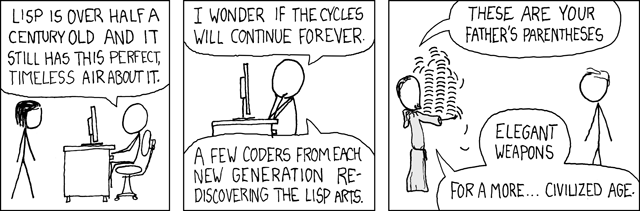
\includegraphics[width=4.25in]{images/lisp_cycles.png} \\
\subcaps{\url{xkcd}}\index{general}{xkcd}
}

%Lazy evaluation increases the expressiveness of a language by supporting delayed evaluation.  The main disadvantage of lazy evaluation is it makes the evaluation rules more complex.  This makes it 
%somewhat more complex to build an interpreter, but more importantly, makes it more difficult for humans to understand and reason about programs. 



\cut{
\begin{quote}
{\em I think that there is far too much work done in the world, that immense harm is caused by the belief that work is virtuous, and that what needs to be preached in modern industrial countries is quite different from what always has been preached. Everyone knows the story of the traveler in Naples who saw twelve beggars lying in the sun (it was before the days of Mussolini), and offered a lira to the laziest of them. Eleven of them jumped up to claim it, so he gave it to the twelfth. This traveler was on the right lines. But in countries which do not enjoy Mediterranean sunshine idleness is more difficult, and a great public propaganda will be required to inaugurate it. \ldots All this is only preliminary. I want to say, in all seriousness, that a great deal of harm is being done in the modern world by belief in the virtuousness of work, and that the road to happiness and prosperity lies in an organized diminution of work.

First of all: what is work? Work is of two kinds: first, altering the position of matter at or near the earth's surface relatively to other such matter; second, telling other people to do so. The first kind is unpleasant and ill paid; the second is pleasant and highly paid. The second kind is capable of indefinite extension: there are not only those who give orders, but those who give advice as to what orders should be given. Usually two opposite kinds of advice are given simultaneously by two organized bodies of men; this is called politics.}
\flushright Bertrand Russell, \emph{In Praise of Idleness}, 1932
\end{quote}
}

\LATER{more advantages and disadvantages}

\LATER{preview next chapter}






\LATER{Add evaluation rules for Charme?}





